%%%%%%%%%%%%%%%%%%%%%%%%%%%%%%%%%%%%%%%%%%%%%%%%%%%%%%
% A Beamer template for Ritsumeikan University       %
% Author: Ming-Hao Xu (Xu Minghao)                   %
% Date:   April 2022.                                %
% LPPL Licensed.                                     %
%%%%%%%%%%%%%%%%%%%%%%%%%%%%%%%%%%%%%%%%%%%%%%%%%%%%%%

\documentclass{beamer}
\usepackage{hyperref}

\usepackage[UTF8]{ctex}
\usepackage[T1]{fontenc}

% other packages
\usepackage{latexsym,amsmath,xcolor,multicol,booktabs,calligra}
\usepackage{graphicx,pstricks,listings,stackengine}
\usefonttheme[onlymath]{serif}

% dummy text; remove it when working on this template
\usepackage{lipsum}

\author{Ebola}
\title{字符串进阶:扩展kmp}
\institute{
    Institute of Mathematics, \\
    Zhejiang University.
}
\date{Jan, 2024}
\usepackage{Ritsumeikan}

% defs
\def\cmd#1{\texttt{\color{red}\footnotesize $\backslash$#1}}
\def\env#1{\texttt{\color{blue}\footnotesize #1}}
\definecolor{deepblue}{rgb}{0,0,0.5}
\definecolor{deepred}{rgb}{0.6,0,0}
\definecolor{deepgreen}{rgb}{0,0.5,0}
\definecolor{halfgray}{gray}{0.55}

\lstset{
    basicstyle=\ttfamily\tiny,
    keywordstyle=\bfseries\color{deepblue},
    emphstyle=\ttfamily\color{deepred},    % Custom highlighting style
    stringstyle=\color{deepgreen},
    numbers=left,
    numberstyle=\small\color{halfgray},
    rulesepcolor=\color{red!20!green!20!blue!20},
    frame=shadowbox,
}


\begin{document}

\begin{frame}
    \titlepage
\end{frame}

\begin{frame}
    \tableofcontents[sectionstyle=show,subsectionstyle=show/shaded/hide,subsubsectionstyle=show/shaded/hide]
\end{frame}

\section{基础回顾}

\begin{frame}{kmp算法}
    \small

    kmp算法解决的是单文本串、单模式串匹配问题,即:
    给定文本串 $S$ 和模式串 $T$,求 $T$ 在 $S$ 中完整出现的所有位置。

    \vspace{1em}
    复杂度是 $O(n)$.
\end{frame}

\begin{frame}[fragile]{kmp算法}
    \footnotesize
    我们来回顾一下 kmp 算法的流程。
    首先有一个 next 数组,我这里把它写成 $\pi$,定义如下:
    \begin{equation*}
        \pi(i)=\max \{k\;|\; T[1,...,k]=T[i-k+1,...,i],\; k=0,...,i-1\}
    \end{equation*}

    \vspace{1em}\pause
    我们把 $T$(长$m$) 和 $S$(长$n$,$n>m$) 放到一起:
    \verb|A = T#S|
    
    \vspace{1em}
    对于一个位置 $i$,如果 $\pi(i)=m$,说明 $T$ 从 $i-m+1$ 位置开始出现;
    反过来,如果 $T$ 从 $i-m+1$ 位置开始出现,那么一定 $\pi(i)=m$。
    
    \vspace{1em}
    我们只要找到 $\pi(i)=m$ 的位置,然后就知道答案了。
\end{frame}

\begin{frame}[fragile]{kmp算法}
    \footnotesize
    现在考虑如何求 $\pi$ 数组。

    最暴力的求法,$O(n^3)$:

    \begin{lstlisting}[language=c++]
for(int i = 1; i <= n; i++){
    int k;
    for(k = i-1; k >= 0; k--)
        if(子串(1,...,k) == 子串(i-k+1,...,i))
            break;
    pi[i] = k;
}
    \end{lstlisting}
\end{frame}

\begin{frame}[fragile]{kmp算法}
    \footnotesize
    我们观察到:$\pi(i+1)\leq \pi(i)+1$,为什么?(举例说明)

    \vspace{1em}\pause
    借助这个观察,我们可以优化代码:
    \begin{lstlisting}[language=c++]
for(int i = 1; i <= n; i++){
    int k;
    for(k = pi[i-1]+1; k >= 0; k--)
        if(子串(1,...,k) == 子串(i-k+1,...,i))
            break;
    pi[i] = k;
}
    \end{lstlisting}

    这个复杂度是 $O(n^2)$
\end{frame}

\begin{frame}[fragile]{kmp算法}
    \footnotesize
    现在我们看这个集合:
    \begin{equation*}
        \mathcal{P}(i)=\{k\;|\; T[1,...,k]=T[i-k+1,...,i],\; k=0,...,i-1\}.
    \end{equation*}
    注意到 $\pi(i)=\max \mathcal{P}(i)$.

    \vspace{1em}\pause
    又注意到 $\pi(i)-1\in\mathcal{P}(i-1)$(为什么?)。
    \pause 那么 $k$ 循环可以只遍历 $\mathcal{P}(i-1)$ 里的数,像这样:

    \begin{lstlisting}[language=c++]
pi[1] = 0;
for(int i = 2; i <= n; i++){
    int k;
    for(k = max(P(i-1)); k >= 0; k=P(i-1)里面比k小的那个数)
        if(A[k+1] == A[i])
            break;
    pi[i] = k + 1;
}
    \end{lstlisting}

    \vspace{1em}\pause
    注意到 $\mathcal{P}(i)$ 里面第二大的数是 $\pi(\pi(i))$,
    第三大的数是 $\pi(\pi(\pi(i)))$,…… (为什么?)
    所以上面的 $k$ 循环很好实现。总复杂度 $O(n)$.
\end{frame}

\begin{frame}{[HNOI2008] GT考试}

    \small 
    阿申准备报名参加 GT 考试,准考证号为 $N$ 位数$X_1,X_2…X_n\ (0\le X_i\le 9)$,他不希望准考证号上出现不吉利的数字。
    
    \vspace{1em}
    他的不吉利数字$A_1,A_2,\cdots, A_m\ (0\le A_i\le 9)$ 有 $M$ 位,不出现是指 $X_1,X_2\cdots X_n$ 中没有恰好一段等于 $A_1,A_2,\cdots ,A_m$,$A_1$ 和 $X_1$ 可以为 $0$。

    \vspace{1em}
    阿申想知道不出现不吉利数字的号码有多少种,输出模 $K$ 取余的结果。

    \vspace{1em}
    $N\leq10^9$,$M\leq 20$,$K\leq1000$。
\end{frame}

\begin{frame}{[HNOI2008] GT考试}
    \small 
    设 $f_{i,j}$ 表示当前考虑到第 $i$ 位,其中末尾和 $A_1...A_m$ 匹配了 $j$ 位。

    设 $g_{j,k}$ 表示当前末尾匹配了 $j$ 位,如果添加一个数字后能够匹配 $k$ 位,
    有多少种添加数字的方案。这是一个可以预处理的数组。

    \vspace{1em}\pause
    我们得到转移方程:
    \begin{equation*}
        f_{i,j}=\sum_{k=0}^{m-1} f_{i-1,k}g_{k,j}.
    \end{equation*}

    显然可以用矩阵快速幂优化(应该都会吧?)。

    \vspace{1em}\pause
    $g$ 数组可以用 kmp 来算。枚举当前匹配长度 $j$,再枚举下一个数字 $c$,
    用 next 数组算一下添加 $c$ 之后末尾匹配长度是多少(记为 $k$),然后令 $g_{j,k}++$.
\end{frame}

\section{扩展 kmp (Z 函数)}

\begin{frame}{扩展 kmp (Z 函数)}
    \small

    对于一个长度为 $n$ 的字符串,定义 $z_i$ 表示 $s$ 与 $s[i...n]$ 的最长公共前缀长度。
    这就是 \textbf{Z 函数}。
\end{frame}

\begin{frame}[fragile]{扩展 kmp (Z 函数)}
    \small

    朴素求法是 $O(n^2)$ 的,像这样:

    \begin{lstlisting}[language=c++]
void get_z(char s[], int n, int z[]) {
    z[1] = n;
    for(int i = 2; i <= n; i++){
        z[i] = 0;
        while(i + z[i] - 1 < n && s[1 + z[i]] == s[i + z[i]]) z[i]++;
    }
}
    \end{lstlisting}

    在学习线性算法之前,我们先来看几个简单的应用。
\end{frame}

\begin{frame}[fragile]{字符串匹配}
    \small

    给定文本串 $S$ 和模式串 $T$,求 $T$ 在 $S$ 中完整出现的所有位置。

    \pause\vspace{1em}
    【解】令 \verb|A=T#S|,求出 $A$ 的 Z 函数,然后找到所有 $z_i=|T|$ 的位置即可。
\end{frame}

\begin{frame}[fragile]{本质不同的子串}
    \small

    给定文本串 $S$,现在往 $S$ 的开头添加一个字母 $c$,
    问增加了几个本质不同的子串。

    \pause\vspace{1em}
    【解】求 $cS$ 的 Z 函数,取最大值 $z_\text{max}$,显然,
    长度超过 $z_\text{max}$ 的前缀都是新增的本质不同子串(反之,
    长度不超过 $z_\text{max}$ 的前缀都不是新增的本质不同子串)。
\end{frame}

\begin{frame}[fragile]{字符串的最小周期(UVA455 加强版)}
    \small
    给定一个长度为 $n\;(\leq 10^7)$ 的字符串 $S$,
    找到其最短的整周期,
    即寻找一个最短的字符串 $T$,
    使得 $S$ 可以被若干个 $T$ 拼接而成的字符串表示。

    \pause\vspace{1em}
    【解】求 $S$ 的 Z 函数,找到最小的 $n$ 的因数 $i$,满足 $i+z_{i+1}=n$.
\end{frame}

\begin{frame}[fragile]{最长回文前缀}
    \small
    给定一个长度为 $n\;(\leq 10^7)$ 的字符串 $S$,
    求一个最长的字符串 $T$,使 $T$ 既是回文又是 $S$ 的前缀。

    \pause\vspace{1em}
    【解】把 $S$ 翻转过来得到 $S'$,然后令 \verb|A=S#S'|。
    找到第一个位置 $i>n$,满足 $i+z_{i}-1=2n+1$.
\end{frame}

\begin{frame}[fragile]{Z 函数的线性算法}
    \footnotesize
    我们称区间 $[i,i+z_i-1]$ 为 $i$ 的 Z-box.

    \vspace{1em}\pause
    我们维护右端点最靠右的 Z-box,记作 $[l,r]$。根据定义,$S[l,r]$ 是 $S$ 的前缀。
    在计算 $z_i$ 时我们保证 $l\leq i$,初始时 $l=r=1$.

    \vspace{1em}
    现在来计算 $z_i$。

    \pause\vspace{.5em}\textbf{Case 1}($i\leq r$):此时有 $S[i,r]=S[i-l+1,r-l+1]$.
    \begin{figure}[H]
        \centering
        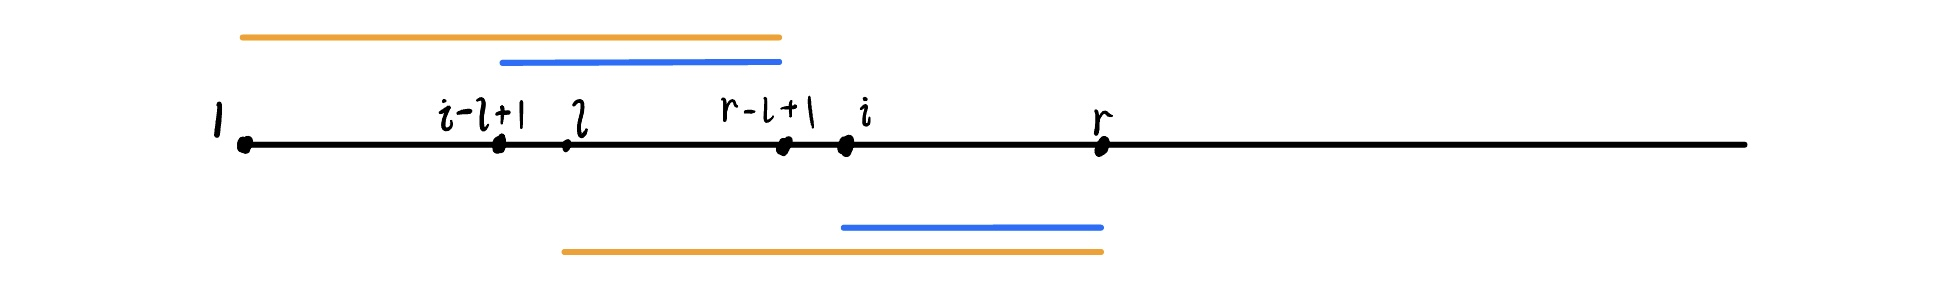
\includegraphics[width=\textwidth]{pic/exkmp-1.jpg}
    \end{figure}

    显然,$z_i\geq \min(z_{i-l+1},r-i+1)$. 此时:
    \begin{itemize}
        \pause \item 若 $z_{i-l+1}<r-i+1$,则 $z_i=z_{i-l+1}$,无法继续扩展;
        \pause \item 否则,我们令 $z_i=r-i+1$,然后暴力枚举下一个字符扩展 $z_i$。
    \end{itemize}

    \pause\vspace{.5em}\textbf{Case 2}($i> r$):此时从 $S[i]$ 开始暴力枚举。

    \pause\vspace{.5em}\textbf{注意}:如果求出 $z_i$ 后发现 $i+z_i-1>r$,则需要更新 $[l,r]$.(\href{https://personal.utdallas.edu/~besp/demo/John2010/z-algorithm.htm}{在线模拟})
\end{frame}

\begin{frame}[fragile]{Z 函数的线性算法}
    \small
    \begin{lstlisting}[language=c++]
void get_z(char s[], int z[]){
    int n = strlen(s+1);
    int l = 1, r = 1;
    for(int i = 2; i <= n; i++){
        z[i] = (i <= r) ? min(z[i-l+1], r-i+1) : 0;
        // 注意:当 i<=r 且 z[i-l+1]<r-i+1 时,while 循环一定不会执行
        while(i+z[i] <= n && s[1+z[i]] == s[i+z[i]]) z[i]++;
        if(i+z[i]-1 > r) l = i, r = i+z[i]-1;
    }
    z[1] = n;
}
    \end{lstlisting}

    \vspace{1em}\pause
    为什么这个算法是 $O(n)$ 的?

    \vspace{1em}\pause
    【答】每执行一次 \verb|while| 循环,必然导致 $r$ 向后移动至少一位。
    而 $r\leq n$,所以总共最多执行 $n$ 次。
\end{frame}

\begin{frame}[fragile]{【模板】扩展KMP}
    \small
    给定两个字符串 $a,b$,长度 $\leq 2\times 10^7$,你要求出两个数组:

    \begin{itemize}
        \item $b$ 的 $z$ 函数数组 $z$,即 $b$ 与 $b$ 的每一个后缀的 LCP 长度。
        \item $b$ 与 $a$ 的每一个后缀的 LCP 长度数组 $p$。
    \end{itemize}

    对于一个长度为 $n$ 的数组 $a$,设其权值为 $\operatorname{xor}_{i=1}^n i \times (a_i + 1)$。

    \vspace{1em}
    注:LCP,即 Longest Common Prefix, 最长公共前缀。

    \vspace{1em}\pause

    【解】令 \verb|c=b#a|,求它的 Z 函数 $z^c$ 即可。$z^b_i=z^c_i$,$p_i=z^c_{|b|+1+i}$.
\end{frame}

\begin{frame}[fragile]{[UVA11475] Extend to Palindrome}
    \small
    给定一个字符串 $S$,在其末尾添加尽可能少的字符,使之成为回文串。
\end{frame}

\begin{frame}[fragile]{[UVA11475] Extend to Palindrome}
    \small
    设 $S'$ 是 $S$ 的反串,显然,答案不会比 $SS'$ 更长。
    我们可以在 $SS'$ 的基础上,从 $S'$ 的开头部分删去尽可能多的东西。

    \vspace{1em}\pause
    我们把 $S$ 拆分,记为 $S=AT$,那么 $S'=T'A'$。
    我们可以考虑将 $T'$ 删去,从而得到 $ATA'$,为了让它是一个回文串,
    $T$ 必须是一个回文串。

    \vspace{1em}\pause
    问题转化成了:求 $S$ 的一个尽可能长的后缀,且它恰好是一个回文串。
    这和我们之前讲的是一样的。
\end{frame}

\begin{frame}[fragile]{[CF432D] Prefixes and Suffixes}
    \small
    给你一个长度为n的长字符串,“完美子串”既是它的前缀也是它的后缀,
    求“完美子串”的个数且统计这些子串的在长字符串中出现的次数
\end{frame}

\begin{frame}[fragile]{[CF432D] Prefixes and Suffixes}
    \small
    如果 $i+z_i-1=n$,那么 $S[i,n](=S[1,n-i+1])$ 就是一个完美子串。如何统计出现次数?

    \vspace{1em}\pause
    只需要统计每个前缀作为子串的出现次数,记第 $i$ 个前缀的出现次数是 \verb|cnt[i]|。
    对于一个位置 $i$,有 $S[i,i]=S[1,1],...,S[i,i+z_i-1]=S[1,z_i]$,
    所以令 \verb|cnt[1]++|,...,\verb|cnt[z[i]]++| 即可。

    \vspace{1em}\pause
    不需要对每个 $i$ 都从 $1$ 枚举到 $z_i$ 去统计,
    只要令 \verb|cnt[z[i]]++|,最后对 \verb|cnt| 数组做一次后缀和即可。
\end{frame}

\begin{frame}[fragile]{[UVA11022] String Factoring(加强版)}
    \small
    我们可以把字符串中连续几个相同的部分压缩成相同的一个。
    压缩可以嵌套进行,比如字符串 $DOODOO$ 可以先压缩成 $(DOO)^2$,然后压缩成 $(D(O)^2)^2$。

    \vspace{1em}
    一个字符串的 Factoring 是它经过若干次压缩得到的结果,
    这个结果不能再次压缩。比如 $(DOO)^2$ 就不是 $DOODOO$ 的压缩,
    因为 $(DOO)^2$ 还可以进一步压缩成 $(D(O)^2)^2$。
    给定字符串 $S$(长度不超过 500 且仅包含大写英文字母),
    求出它的最短 Factoring 的长度。
\end{frame}

\begin{frame}[fragile]{[UVA11022] String Factoring(加强版)}
    \small
    区间 dp,设 $f_{l,r}$ 表示区间 $[l,r]$ 的答案。分两种情况:

    \begin{enumerate}
        \pause \item 直接压缩:找到 $S[l,r]$ 的最小循环节 $S[l,c]$,令 $f_{l,r}=f_{l,c}$.
        \pause \item 分段压缩:找一个分界点 $k$,对两侧分别压缩,即令 $f_{l,r}=\min(f_{l,r},f_{l,k}+f_{k+1,r})$.
    \end{enumerate}

    \pause 对于第一种情况,可以借助 Z 函数 $O(r-l)$ 完成,因此总复杂度 $O(n^3)$.
\end{frame}

\begin{frame}[fragile]{[CODECHEF] Chef and String}
    \small
    给定一个字符串 $S$,多组询问,每次给定一个整数 $k$,问
    在 $S$ 的所有子串中挑选出 $k$ 个完全一样的字符串有几种方案。
    对 $10^9+7$ 取模。

    \vspace{1em}
    例如 $S="ababa"$,$k=2$,则答案为 $7$.

    \vspace{1em}
    字符串长度 $\leq 5000$,询问总数 $\leq 10^5$.
\end{frame}

\begin{frame}[fragile]{[CODECHEF] Chef and String}
    \small
    如果我们知道出现 $i$ 次的本质不同子串有多少个,记作 $f_i$,那么
    对于给定 $k$ 的询问,答案就是:
    \begin{equation*}
        \text{ans}_k=\sum_{i=k}^n f_i \binom{i}{k}.
    \end{equation*}

    如果数组 $f$ 已知,我们可以 $O(n^2)$ 算出 $\text{ans}_1,...,\text{ans}_n$,
    然后 $O(1)$ 回答每个询问。

    \vspace{1em}\pause
    现在来考虑如何计算数组 $f$。
\end{frame}

\begin{frame}[fragile]{[CODECHEF] Chef and String}
    \small
    问题:求出现 $i$ 次的本质不同子串有多少个($f_i$)。

    \vspace{1em}\pause
    由于本质不同子串总共最多 $\frac{1}{2}n^2$ 个,
    我们可以给它们编一个号,用数组 \verb|idx[l][r]| 来表示 $S[l,r]$
    是第几个本质不同子串。然后用 \verb|cnt[i]| 
    表示第 $i$ 个本质不同子串出现了几次。

    \vspace{1em}\pause
    可以发现 \verb|cnt| 是 \verb|idx| 的桶,\verb|f| 又是 \verb|cnt| 的桶。

    \begin{lstlisting}[language=c++]
for(int i = 1; i <= n; i++)
    for(int j = i; j <= n; j++)
        cnt[idx[i][j]]++;
for(int i = 1; i <= maxidx; i++)
    f[cnt[i]]++;
    \end{lstlisting}

    现在关键是求出 \verb|idx| 数组。
\end{frame}

\begin{frame}[fragile]{[CODECHEF] Chef and String}
    \small
    问题:求 \verb|idx[l][r]| 表示 $S[l,r]$ 是第几个本质不同的子串。
    (内容相同但位置不同的子串应该有相同的编号)

    \vspace{1em}\pause
    我们从后往前求,首先令 \verb|idx[n][n]=1|. 接下来我们依次往前添加字符。
    \pause 假设现在已经求完了 \verb|idx[l][r]| $(i<l\leq r)$,我们要求出 \verb|idx[i][r]| $(i\leq r\leq n)$.

    \vspace{1em}\pause
    我们令 $T=S[i,n]$,求出 $T$ 的 Z 数组 $z_1,...,z_{n-i+1}$. 找到最大值 $z_j=\max\{z_1,...,z_{n-i+1}\}$.

    \vspace{1em}\pause
    现在,$S[i,i],...,S[i,i+z_j-1]$ 都是在后面出现过的子串,所以令 \verb|idx[i][i+k]=idx[i+j-1][i+j-1+k]| ($0\leq k < z_j$).
    \vspace{.5em}
    而 $S[i,i+z_j],...,S[i,n]$ 都是新增的本质不同子串,给它们新的编号即可。
\end{frame}

\begin{frame}[fragile]{[NOIP2020] 字符串匹配}
    \footnotesize
    小 C 学习完了字符串匹配的相关内容,现在他正在做一道习题。

    \vspace{.5em}
    对于一个字符串 $S$,题目要求他找到 $S$ 的所有具有下列形式的拆分方案数:

    \vspace{.5em}
    $S = ABC$,$S = ABABC$,$S = ABAB \ldots ABC$,其中 $A$,$B$,$C$ 均是非空字符串,且 $A$ 中出现奇数次的字符数量不超过 $C$ 中出现奇数次的字符数量。

    \vspace{.5em}
    更具体地,我们可以定义 $AB$ 表示两个字符串 $A$,$B$ 相连接,例如 $A = \texttt{aab}$,$B = \texttt{ab}$,则 $AB = \texttt{aabab}$。

    \vspace{.5em}
    并递归地定义 $A^1=A$,$A^n = A^{n - 1} A$($n \ge 2$ 且为正整数)。例如 $A = \texttt{abb}$,则 $A^3=\texttt{abbabbabb}$。

    \vspace{.5em}
    则小 C 的习题是求 $S = {(AB)}^iC$ 的方案数,其中 $F(A) \le F(C)$,$F(S)$ 表示字符串 $S$ 中出现奇数次的字符的数量。两种方案不同当且仅当拆分出的 $A$、$B$、$C$ 中有至少一个字符串不同。

    \vspace{.5em}
    小 C 并不会做这道题,只好向你求助,请你帮帮他。
\end{frame}

\begin{frame}[fragile]{[NOIP2020] 字符串匹配}
    \footnotesize
    我们构造两个辅助数组:\verb|suf[p]|$=F(S[p,n])$,
    \verb|f[p][c]| 表示 $F(S[1,1]),F(S[1,2]),...,F(S[1,p])$ 中 $\leq c$ 的数有几个。

    \vspace{.5em}
    我们先别管怎么求这两个数组,假如已经求出来了,我们应该如何计算答案?

    \vspace{.5em}\pause
    我们可以枚举 $AB=S[1,p]$,然后枚举 $i$,那么 $(AB)^i=S[1,ip]$,$C=S[ip+1,n]$.
    由于我们要保证 $S[1,p]$ 是 $S[1,ip]$ 的循环节,因此必须满足 $ip\leq p+z_{p+1}$(为什么?);
    当然,为了保证 $C$ 非空,还要满足 $ip\leq n-1$.

    \vspace{.5em}\pause
    现在,我们要考虑将 $S[1,p]$ 拆分成 $A$ 和 $B$,并且保证 $F(A)\leq F(C)$,
    以及 $A,B$ 均非空,那么方案有多少种?
    \pause(答案是 \verb|f[p-1][suf[i*p+1]]|).

    \pause
    \begin{lstlisting}[language=c++]
long long ans = 0;
// 枚举 AB = S[1,p]
for(int p = 2; p < n; p++){
    int ed = min(p + z[p+1], n-1);
    // 枚举 (AB)^i 中的 i
    for(int i = 1; i * p <= ed; i++)
        // 寻找 S[1,p] 有几种划分成 AB 的方案使得 F(A)<=F(C)
        ans += f[p-1][suf[i * p + 1]];
}
    \end{lstlisting}
    复杂度:$\sum_{p=1}^n O(\frac{n}{p})=O(n\ln n)$.
\end{frame}

\begin{frame}[fragile]{[NOIP2020] 字符串匹配}
    \footnotesize
    现在来思考如何求辅助数组:\verb|suf[p]|$=F(S[p,n])$,以及
    \verb|f[p][c]| 表示 $F(S[1,1]),F(S[1,2]),...,F(S[1,p])$ 中 $\leq c$ 的数有几个。

    \vspace{1em}\pause
    \verb|suf[p]| 非常好求,直接看代码
    \begin{lstlisting}[language=c++]
suf[n+1] = 0;
memset(cnt, 0, sizeof(cnt));
for(int p = n; p >= 1; p--){
    cnt[s[p]-'a']++;
    if(cnt[s[p]-'a'] & 1) suf[p] = suf[p+1] + 1;
    else suf[p] = suf[p+1] - 1;
}
    \end{lstlisting}
    这是因为 $F(S[p,n])=F(S[p+1,n])\pm 1$,加一还是减一由 $S[p]$ 在 $S[p,n]$ 中出现的次数决定。

    \vspace{1em}\pause
    事实上,为了求出 \verb|f[p][c]| 数组,我们还需要一个辅助数组:\verb|pre[p]|$=F(S[1,p])$,
    现在请大家仿照上面的代码写出求 \verb|pre| 的代码。
\end{frame}

\begin{frame}[fragile]{[NOIP2020] 字符串匹配}
    \footnotesize
    现在,我们先统计 $F(S[1,1]),...,F(S[1,p])$ 中 $=c$ 的数有几个。
    \begin{lstlisting}[language=c++]
for(int p = 1; p <= n; p++){
    memcpy(f[p], f[p-1], sizeof(f[p]));
    f[p][pre[p]]++;
}
    \end{lstlisting}

    \vspace{1em}\pause
    再对 $c$ 做一个前缀和,就得到了我们需要的 \verb|f[p][c]|.
    \begin{lstlisting}[language=c++]
for(int p = 1; p <= n; p++)
    for(int c = 1; c <= 26; c++)
        f[p][c] += f[p][c-1];
    \end{lstlisting}
\end{frame}

\begin{frame}
    \begin{center}
        {\Huge\calligra Thank You}
    \end{center}
\end{frame}

\end{document}